\documentclass[aspectratio=169]{beamer}\usepackage[]{graphicx}\usepackage[]{xcolor}
% maxwidth is the original width if it is less than linewidth
% otherwise use linewidth (to make sure the graphics do not exceed the margin)
\makeatletter
\def\maxwidth{ %
  \ifdim\Gin@nat@width>\linewidth
    \linewidth
  \else
    \Gin@nat@width
  \fi
}
\makeatother

\definecolor{fgcolor}{rgb}{0.345, 0.345, 0.345}
\newcommand{\hlnum}[1]{\textcolor[rgb]{0.686,0.059,0.569}{#1}}%
\newcommand{\hlsng}[1]{\textcolor[rgb]{0.192,0.494,0.8}{#1}}%
\newcommand{\hlcom}[1]{\textcolor[rgb]{0.678,0.584,0.686}{\textit{#1}}}%
\newcommand{\hlopt}[1]{\textcolor[rgb]{0,0,0}{#1}}%
\newcommand{\hldef}[1]{\textcolor[rgb]{0.345,0.345,0.345}{#1}}%
\newcommand{\hlkwa}[1]{\textcolor[rgb]{0.161,0.373,0.58}{\textbf{#1}}}%
\newcommand{\hlkwb}[1]{\textcolor[rgb]{0.69,0.353,0.396}{#1}}%
\newcommand{\hlkwc}[1]{\textcolor[rgb]{0.333,0.667,0.333}{#1}}%
\newcommand{\hlkwd}[1]{\textcolor[rgb]{0.737,0.353,0.396}{\textbf{#1}}}%
\let\hlipl\hlkwb

\usepackage{framed}
\makeatletter
\newenvironment{kframe}{%
 \def\at@end@of@kframe{}%
 \ifinner\ifhmode%
  \def\at@end@of@kframe{\end{minipage}}%
  \begin{minipage}{\columnwidth}%
 \fi\fi%
 \def\FrameCommand##1{\hskip\@totalleftmargin \hskip-\fboxsep
 \colorbox{shadecolor}{##1}\hskip-\fboxsep
     % There is no \\@totalrightmargin, so:
     \hskip-\linewidth \hskip-\@totalleftmargin \hskip\columnwidth}%
 \MakeFramed {\advance\hsize-\width
   \@totalleftmargin\z@ \linewidth\hsize
   \@setminipage}}%
 {\par\unskip\endMakeFramed%
 \at@end@of@kframe}
\makeatother

\definecolor{shadecolor}{rgb}{.97, .97, .97}
\definecolor{messagecolor}{rgb}{0, 0, 0}
\definecolor{warningcolor}{rgb}{1, 0, 1}
\definecolor{errorcolor}{rgb}{1, 0, 0}
\newenvironment{knitrout}{}{} % an empty environment to be redefined in TeX

\usepackage{alltt}

% Set lecture number for later use


% Part common to all the lectures
\subtitle{MATH 2740 -- Mathematics of Data Science -- Lecture 14}
\author{\texorpdfstring{Julien Arino\newline\url{julien.arino@umanitoba.ca}}{Julien Arino}}
\institute{Department of Mathematics @ University of Manitoba}
\date{Fall 202X}

% Title of the lecture
\title{Matrix methods -- Support vector machines}



\usetheme{default}
% Slide setup, colour independent

\usepackage{amsmath,amssymb,amsthm}
\usepackage[utf8]{inputenc}
\usepackage{colortbl}
\usepackage{bm}
\usepackage{xcolor}
\usepackage{dsfont}
\usepackage{setspace}
% To use \ding{234} and the like
\usepackage{pifont}
% To cross reference between slide files
\usepackage{zref-xr,zref-user}
% Use something like
% \zexternaldocument{fileI}
% in the tex files. And cite using \zref instead of \ref

% Cross-reference system - see CROSS-REFERENCE-SETUP.md for manual setup instructions
\usepackage{booktabs}
\usepackage{marvosym}
\usepackage{cancel}
%\usepackage{transparent}
% Make doi clickable in the bibliography?
\usepackage{doi}

\usepackage[T1]{fontenc}

\usepackage{longtable}

% For heavier titles
\usepackage{helvet} % Enables Helvetica font family


% Fields and the like
\def\IC{\mathbb{C}}
\def\IE{\mathbb{E}}
\def\IF{\mathbb{F}}
\def\II{\mathbb{I}}
\def\IJ{\mathbb{J}}
\def\IK{\mathbb{K}}
\def\IM{\mathbb{M}}
\def\IN{\mathbb{N}}
\def\IP{\mathbb{P}}
\def\IR{\mathbb{R}}
\newcommand{\IRplus}{\mathbb{R}_{\ge 0}}
\def\IZ{\mathbb{Z}}
\def\11{\mathds{1}}


% Bold lowercase
\def\ba{\bm{a}}
\def\bb{\bm{b}}
\def\bc{\bm{c}}
\def\bd{\bm{d}}
\def\be{\bm{e}}
\def\bf{\bm{f}}
\def\bg{\bm{g}}
\def\bh{\bm{h}}
\def\bi{\bm{i}}
\def\bj{\bm{j}}
\def\bk{\bm{k}}
\def\bn{\bm{n}}
\def\bp{\bm{p}}
\def\br{\bm{r}}
\def\bs{\bm{s}}
\def\bu{\bm{u}}
\def\bv{\bm{v}}
\def\bw{\bm{w}}
\def\bx{\bm{x}}
\def\by{\bm{y}}
\def\bz{\bm{z}}
\newcommand{\vect}[1]{\bm{#1}}

% Bold capitals
\def\bB{\bm{B}}
\def\bD{\bm{D}}
\def\bE{\bm{E}}
\def\bF{\bm{F}}
\def\bG{\bm{G}}
\def\bI{\bm{I}}
\def\bL{\bm{L}}
\def\bN{\bm{N}}
\def\bP{\bm{P}}
\def\bR{\bm{R}}
\def\bS{\bm{S}}
\def\bT{\bm{T}}
\def\bX{\bm{X}}

% Bold numbers
\def\b0{\bm{0}}

% Bold greek
\bmdefine{\bmu}{\bm{\mu}}
\def\bphi{\bm{\phi}}
\def\bvarphi{\bm{\varphi}}
\def\bPi{\bm{\Pi}}
\def\bGamma{\bm{\Gamma}}

% Bold red sentence
\def\boldred#1{{\color{red}\textbf{#1}}}
\def\defword#1{{\color{orange}\textbf{#1}}}

% Caligraphic letters
\def\A{\mathcal{A}}
\def\B{\mathcal{B}}
\def\C{\mathcal{C}}
\def\D{\mathcal{D}}
\def\E{\mathcal{E}}
\def\F{\mathcal{F}}
\def\G{\mathcal{G}}
\def\H{\mathcal{H}}
\def\I{\mathcal{I}}
\def\L{\mathcal{L}}
\def\M{\mathcal{M}}
\def\N{\mathcal{N}}
\def\P{\mathcal{P}}
\def\R{\mathcal{R}}
\def\S{\mathcal{S}}
\def\T{\mathcal{T}}
\def\U{\mathcal{U}}
\def\V{\mathcal{V}}

% Adding space for prime (') where needed
\def\pprime{\,'}
% Adding space for star (\star) where needed
\def\pstar{{\,\star}}

% tt font for code
\def\code#1{{\tt #1}}

% i.e., e.g.
\def\eg{\emph{e.g.}}
\def\ie{\emph{i.e.}}


% Operators and special symbols
\def\nbOne{{\mathchoice {\rm 1\mskip-4mu l} {\rm 1\mskip-4mu l}
{\rm 1\mskip-4.5mu l} {\rm 1\mskip-5mu l}}}
\def\cov{\ensuremath{\mathsf{cov}}}
\def\Var{\ensuremath{\mathsf{Var}\ }}
\def\Im{\textrm{Im}\;}
\def\Re{\textrm{Re}\;}
\def\det{\ensuremath{\mathsf{det}}}
\def\diag{\ensuremath{\mathsf{diag}}}
\def\nullspace{\ensuremath{\mathsf{null}}}
\def\nullity{\ensuremath{\mathsf{nullity}}}
\def\rank{\ensuremath{\mathsf{rank}}}
\def\range{\ensuremath{\mathsf{range}}}
\def\sgn{\ensuremath{\mathsf{sgn}}}
\def\Span{\ensuremath{\mathsf{span}}}
\def\tr{\ensuremath{\mathsf{tr}}}
\def\imply{$\Rightarrow$}
\def\restrictTo#1#2{\left.#1\right|_{#2}}
\newcommand{\parallelsum}{\mathbin{\!/\mkern-5mu/\!}}
\def\dsum{\mathop{\displaystyle \sum }}%
\def\dind#1#2{_{\substack{#1\\ #2}}}

\newcommand{\Qmatrix}[1]{%
  \begin{pmatrix}#1\end{pmatrix}%
}

\DeclareMathOperator{\GL}{GL}
\DeclareMathOperator{\Rel}{Re}
\def\Nt#1{\left|\!\left|\!\left|#1\right|\!\right|\!\right|}
\newcommand{\tripbar}{|\! |\! |}



% The beamer bullet (in base colour)
\def\bbullet{\leavevmode\usebeamertemplate{itemize item}\ }

% Theorems and the like
\newtheorem{proposition}[theorem]{Proposition}
\newtheorem{property}[theorem]{Property}
\newtheorem{importantproperty}[theorem]{Property}
\newtheorem{importanttheorem}[theorem]{Theorem}
%\newtheorem{lemma}[theorem]{Lemma}
%\newtheorem{corollary}[theorem]{Corollary}
\newtheorem{remark}[theorem]{Remark}
\setbeamertemplate{theorems}[numbered]
%\setbeamertemplate{theorems}[ams style]

%
%\usecolortheme{orchid}
%\usecolortheme{orchid}

\def\red{\color[rgb]{1,0,0}}
\def\blue{\color[rgb]{0,0,1}}
\def\green{\color[rgb]{0,1,0}}

% Fix skipping lines after items in the bibliography
\setbeamertemplate{bibliography entry title}{}
\setbeamertemplate{bibliography entry location}{}
\setbeamertemplate{bibliography entry note}{}

% Get rid of navigation stuff
\setbeamertemplate{navigation symbols}{}

% Set footline/header line
\setbeamertemplate{footline}
{%
\quad p. \insertpagenumber \quad--\quad \insertsection\vskip2pt
}
% \setbeamertemplate{headline}
% {%
% \quad\insertsection\hfill p. \insertpagenumber\quad\mbox{}\vskip2pt
% }


\makeatletter
\newlength\beamerleftmargin
\setlength\beamerleftmargin{\Gm@lmargin}
\makeatother

% Colours for special pages
\def\extraContent{yellow!20}


%%%%%%%%%%%%%%%%%
\usepackage{tikz}
\usetikzlibrary{shapes,arrows}
\usetikzlibrary{positioning}
\usetikzlibrary{shapes.symbols,shapes.callouts,patterns}
\usetikzlibrary{calc,fit}
\usetikzlibrary{backgrounds}
\usetikzlibrary{decorations.pathmorphing,fit,petri}
\usetikzlibrary{automata}
\usetikzlibrary{fadings}
\usetikzlibrary{patterns,hobby}
\usetikzlibrary{backgrounds,fit,petri}
\usetikzlibrary{tikzmark}

\usepackage{pgfplots}
\pgfplotsset{compat=1.6}
\pgfplotsset{ticks=none}

\usetikzlibrary{decorations.markings}
\usetikzlibrary{arrows.meta}
\tikzset{>=stealth}

% For tikz
\tikzstyle{cloud} = [draw, ellipse,fill=red!20, node distance=0.87cm,
minimum height=2em]
\tikzstyle{line} = [draw, -latex']


%%% For max frame images
\newenvironment{changemargin}[2]{%
\begin{list}{}{%
\setlength{\topsep}{0pt}%
\setlength{\leftmargin}{#1}%
\setlength{\rightmargin}{#2}%
\setlength{\listparindent}{\parindent}%
\setlength{\itemindent}{\parindent}%
\setlength{\parsep}{\parskip}%
}%
\item[]}{\end{list}}


% Make one image take up the entire slide content area in beamer,.:
% centered/centred full-screen image, with title:
% This uses the whole screen except for the 1cm border around it
% all. 128x96mm
\newcommand{\titledFrameImage}[2]{
\begin{frame}{#1}
%\begin{changemargin}{-1cm}{-1cm}
\begin{center}
\includegraphics[width=108mm,height=\textheight,keepaspectratio]{#2}
\end{center}
%\end{changemargin}
\end{frame}
}

% Make one image take up the entire slide content area in beamer.:
% centered/centred full-screen image, no title:
% This uses the whole screen except for the 1cm border around it
% all. 128x96mm
\newcommand{\plainFrameImage}[1]{
\begin{frame}[plain]
%\begin{changemargin}{-1cm}{-1cm}
\begin{center}
\includegraphics[width=108mm,height=76mm,keepaspectratio]{#1}
\end{center}
%\end{changemargin}
\end{frame}
}

% Make one image take up the entire slide area, including borders, in beamer.:
% centered/centred full-screen image, no title:
% This uses the entire whole screen
\newcommand{\maxFrameImage}[1]{
\begin{frame}[plain]
\begin{changemargin}{-1cm}{-1cm}
\begin{center}
\includegraphics[width=\paperwidth,height=\paperheight,keepaspectratio]
{#1}
\end{center}
\end{changemargin}
\end{frame}
}

% This uses the entire whole screen (to include in frame)
\newcommand{\maxFrameImageNoFrame}[1]{
\begin{changemargin}{-1cm}{-1cm}
\begin{center}
\includegraphics[width=\paperwidth,height=0.99\paperheight,keepaspectratio]
{#1}
\end{center}
\end{changemargin}
}

% Make one image take up the entire slide area, including borders, in beamer.:
% centered/centred full-screen image, no title:
% This uses the entire whole screen
\newcommand{\maxFrameImageColor}[2]{
\begin{frame}[plain]
\setbeamercolor{normal text}{bg=#2!20}
\begin{changemargin}{-1cm}{-1cm}
\begin{center}
\includegraphics[width=\paperwidth,height=\paperheight,keepaspectratio]
{#1}
\end{center}
\end{changemargin}
\end{frame}
}


\usepackage{tikz}
\usetikzlibrary{patterns,hobby,matrix}
\usepackage{pgfplots}
\pgfplotsset{compat=1.6}
\pgfplotsset{ticks=none}

\usetikzlibrary{backgrounds}
\usetikzlibrary{decorations.markings}
\usetikzlibrary{arrows.meta}
\tikzset{>=stealth}

\tikzset{
  clockwise arrows/.style={
    postaction={
      decorate,
      decoration={
        markings,
        mark=between positions 0.1 and 0.9 step 40pt with {\arrow{>}},
   }}}}


% New integrated section command: creates section and section slide
\newcommand{\Ssection}[2]{
\section{#1}
\begin{frame}[noframenumbering,plain]
  \begin{tikzpicture}[remember picture,overlay]
    \node[above right,inner sep=0pt,opacity=0.2] at (current page.south west)
    {
        \includegraphics[height=\paperheight,width=\paperwidth]{#2}
    };
  \end{tikzpicture}
  \setbeamercolor{section in toc}{fg=section_page_list_colour}
  \setbeamerfont{section in toc}{size=\Large,series=\bfseries}
  \setbeamertemplate{section in toc shaded}[default][60]
  \tableofcontents[
    currentsection,
    sectionstyle=show/shaded,
    subsectionstyle=show/hide/hide,
    subsubsectionstyle=hide/hide/hide]
\end{frame}
\addtocounter{page}{-1}
}

% New integrated section command with subsections: creates section and section slide showing subsections
\newcommand{\SsectionWithSubs}[2]{
\section{#1}
\begin{frame}[noframenumbering,plain]
  \begin{tikzpicture}[remember picture,overlay]
    \node[above right,inner sep=0pt,opacity=0.2] at (current page.south west)
    {
        \includegraphics[height=\paperheight,width=\paperwidth]{#2}
    };
  \end{tikzpicture}
  \setbeamercolor{section in toc}{fg=section_page_list_colour}
  \setbeamerfont{section in toc}{size=\Large,series=\bfseries}
  \setbeamertemplate{section in toc shaded}[default][60]
  \tableofcontents[
    currentsection,
    sectionstyle=show/hide,
    subsectionstyle=show/show/hide,
    subsubsectionstyle=hide/hide/hide]
\end{frame}
\addtocounter{page}{-1}
}

% New integrated subsection command: creates subsection and subsection slide
\newcommand{\Ssubsection}[2]{
\subsection{#1}
\begin{frame}[noframenumbering,plain]
  \begin{tikzpicture}[remember picture,overlay]
    \node[above right,inner sep=0pt,opacity=0.2] at (current page.south west)
    {
        \includegraphics[height=\paperheight,width=\paperwidth]{#2}
    };
  \end{tikzpicture}
  \setbeamercolor{section in toc}{fg=subsection_page_list_colour}
  \setbeamerfont{section in toc}{size=\Large,series=\bfseries}
  \setbeamertemplate{section in toc shaded}[default][60]
  \setbeamerfont{subsection in toc}{series=\bfseries}
  \setbeamertemplate{subsection in toc shaded}[default][50]
  \tableofcontents[
    currentsection,
    sectionstyle=show/hide,
    subsectionstyle=show/shaded/hide,
    subsubsectionstyle=hide/hide/hide]
\end{frame}
\addtocounter{page}{-1}
}

% New integrated subsubsection command: creates subsubsection and subsubsection slide
\newcommand{\Ssubsubsection}[2]{
\subsubsection{#1}
\begin{frame}[noframenumbering,plain]
  \begin{tikzpicture}[remember picture,overlay]
    \node[above right,inner sep=0pt,opacity=0.2] at (current page.south west)
    {
        \includegraphics[height=\paperheight,width=\paperwidth]{#2}
    };
  \end{tikzpicture}
  \setbeamercolor{section in toc}{fg=subsub_header_section}
  \setbeamerfont{section in toc}{size=\Large,series=\bfseries}
  \setbeamertemplate{section in toc shaded}[default][60]
  \setbeamerfont{subsection in toc}{series=\bfseries}
  \setbeamertemplate{subsection in toc shaded}[default][50]
  \setbeamertemplate{subsubsection in toc shaded}[default][50]
  \tableofcontents[
    currentsection,
    sectionstyle=show/hide,
    subsectionstyle=show/hide/hide,
    subsubsectionstyle=show/shaded/hide]
\end{frame}
\addtocounter{page}{-1}
}

% Legacy commands (kept for backward compatibility)
% Beginning of a section
\newcommand{\newSectionSlide}[1]{
\begin{frame}[noframenumbering,plain]
  \begin{tikzpicture}[remember picture,overlay]
    \node[above right,inner sep=0pt,opacity=0.2] at (current page.south west)
    {
        \includegraphics[height=\paperheight,width=\paperwidth]{#1}
    };
  \end{tikzpicture}
  \setbeamercolor{section in toc}{fg=section_page_list_colour}
  \setbeamerfont{section in toc}{size=\Large,series=\bfseries}
  \setbeamertemplate{section in toc shaded}[default][60]
  \tableofcontents[
    currentsection,
    sectionstyle=show/shaded,
    subsectionstyle=show/hide/hide,
    subsubsectionstyle=hide/hide/hide]
\end{frame}
\addtocounter{page}{-1}
}

% Beginning of a section in which we also show subsections
\newcommand{\newSectionWithSubsSlide}[1]{
	\begin{frame}[noframenumbering,plain]
		\begin{tikzpicture}[remember picture,overlay]
			\node[above right,inner sep=0pt,opacity=0.2] at (current page.south west)
			{
				\includegraphics[height=\paperheight,width=\paperwidth]{#1}
			};
		\end{tikzpicture}
		\setbeamercolor{section in toc}{fg=section_page_list_colour}
		\setbeamerfont{section in toc}{size=\Large,series=\bfseries}
		\setbeamertemplate{section in toc shaded}[default][60]
		\tableofcontents[
		currentsection,
		sectionstyle=show/hide,
		subsectionstyle=show/show/hide,
		subsubsectionstyle=hide/hide/hide]
	\end{frame}
	\addtocounter{page}{-1}
}

% Beginning of a subsection
\newcommand{\newSubSectionSlide}[1]{
\begin{frame}[noframenumbering,plain]
  \begin{tikzpicture}[remember picture,overlay]
    \node[above right,inner sep=0pt,opacity=0.2] at (current page.south west)
    {
        \includegraphics[height=\paperheight,width=\paperwidth]{#1}
    };
  \end{tikzpicture}
  \setbeamercolor{section in toc}{fg=subsection_page_list_colour}
  \setbeamerfont{section in toc}{size=\Large,series=\bfseries}
  \setbeamertemplate{section in toc shaded}[default][60]
  \setbeamerfont{subsection in toc}{series=\bfseries}
  \setbeamertemplate{subsection in toc shaded}[default][50]
  \tableofcontents[
    currentsection,
    sectionstyle=show/hide,
    subsectionstyle=show/shaded/hide,
    subsubsectionstyle=hide/hide/hide]
\end{frame}
\addtocounter{page}{-1}
}

% Beginning of a subsubsection
\newcommand{\newSubSubSectionSlide}[1]{
\begin{frame}[noframenumbering,plain]
  \begin{tikzpicture}[remember picture,overlay]
    \node[above right,inner sep=0pt,opacity=0.2] at (current page.south west)
    {
        \includegraphics[height=\paperheight,width=\paperwidth]{#1}
    };
  \end{tikzpicture}
  \setbeamercolor{section in toc}{fg=subsub_header_section}
  \setbeamerfont{section in toc}{size=\Large,series=\bfseries}
  \setbeamertemplate{section in toc shaded}[default][60]
  \setbeamerfont{subsection in toc}{series=\bfseries}
  \setbeamertemplate{subsection in toc shaded}[default][50]
  \setbeamertemplate{subsubsection in toc shaded}[default][50]
  \tableofcontents[
    currentsection,
    sectionstyle=show/hide,
    subsectionstyle=show/hide/hide,
    subsubsectionstyle=show/shaded/hide]
\end{frame}
\addtocounter{page}{-1}
}


   %%%%%%%%%%%
% To have links to parts in the outline
\makeatletter
\AtBeginPart{%
  \addtocontents{toc}{\protect\beamer@partintoc{\the\c@part}{\beamer@partnameshort}{\the\c@page}}%
}
%% number, shortname, page.
\providecommand\beamer@partintoc[3]{%
  \ifnum\c@tocdepth=-1\relax
    % requesting onlyparts.
    \makebox[6em]{Part #1:} \textcolor{green!30!blue}{\hyperlink{#2}{#2}}
    \par
  \fi
}
\define@key{beamertoc}{onlyparts}[]{%
  \c@tocdepth=-1\relax
}
\makeatother%

\newcommand{\nameofthepart}{}
\newcommand{\nupart}[1]%
    {   \part{#1}%
        \renewcommand{\nameofthepart}{#1}%
        {
          \setbeamercolor{background canvas}{bg=orange!50}
          \begin{frame}{#1}%\partpage 
          \hypertarget{\nameofthepart}{}\tableofcontents%
          \end{frame}
        }
    }

% This command creates a title page using TikZ only
\newcommand{\tikztitlepage}[1]{%
\begin{frame}[plain,noframenumbering]
  \begin{tikzpicture}[remember picture,overlay]
    % Background image
    \node[above right,inner sep=0pt,opacity=0.1] 
      at (current page.south west) 
      {\includegraphics[width=\paperwidth,height=\paperheight]{#1}};

    % University logo
    \node[anchor=north east, inner sep=5pt, opacity=0.9] 
      at (current page.north east)
      {
\includegraphics[width=0.2\textwidth]{FIGS-slides-admin/UM-logo-horizontal-CMYK.png}};
    
    % Title
    \node[anchor=center, align=center, 
          font=\fontsize{13}{15}\bfseries\color{UMbrown}, 
          text width=0.9\textwidth] 
          at ([yshift=2cm]current page.center)
          {\inserttitle};

      % Authors
      \node[anchor=center, align=center,
        font=\fontsize{10}{12}\bfseries\color{UMbrown},
        text width=0.7\textwidth]
        at ([yshift=0.8cm]current page.center)
        {\insertauthor};

      % Affiliation
      \node[anchor=north, align=center,
        font=\fontsize{9}{11}\color{UMbrown},
        text width=0.7\textwidth]
        at ([yshift=-0.2cm]current page.center)
        {\insertaffiliation};      
    % Date
    \node[anchor=north, align=center, 
          font=\fontsize{12}{16}\bfseries\color{UMbrown},
          text width=0.7\textwidth] 
          at ([yshift=0.2cm]current page.center)
          {\insertdate};

    % Land acknowledgement
    \node[anchor=south, align=justify, 
          font=\footnotesize, text=black, 
          text width=1.1\textwidth] 
          at ([yshift=0.5cm]current page.south)
          {The University of Manitoba campuses are located on original lands of Anishinaabeg, Ininew, Anisininew, Dakota and Dene peoples, and on the National Homeland of the Red River Métis.\\
          We respect the Treaties that were made on these territories, we acknowledge the harms and mistakes of the past, and we dedicate ourselves to move forward in partnership with Indigenous communities in a spirit of Reconciliation and collaboration.};
  \end{tikzpicture}
  \addtocounter{page}{-1}
\end{frame}
}
% The title page with figure
% \newcommand{\titlepagewithfigure}[1]{%
%   \begin{frame}[noframenumbering,plain]
%     \begin{tikzpicture}[remember picture,overlay]
%       \node[above right,inner sep=0pt,opacity=0.1] at (current page.south west)
%       {
%           \includegraphics[height=\paperheight,width=\paperwidth]{#1}
%       };
%       \node[anchor=north east,
%       inner sep=5pt,
%       opacity=0.9] at (current page.north east)
%       {
%           
\includegraphics[width=0.2\textwidth]{FIGS-slides-admin/UM-logo-horizontal-CMYK.png}
%       };
%       \node[anchor=south, 
%       align=justify, 
%       text=black, 
%       text width=1.1\textwidth,
%       font=\footnotesize]  (land_acknowledgement)
%       at (current page.south) 
%       {The University of Manitoba campuses are located on original lands of Anishinaabeg, Ininew, Anisininew, Dakota and Dene peoples, and on the National Homeland of the Red River Métis.
%       We respect the Treaties that were made on these territories, we acknowledge the harms and mistakes of the past, and we dedicate ourselves to move forward in partnership with Indigenous communities in a spirit of Reconciliation and collaboration.};  
%       % \node[align=center, anchor=south,
%       % above=0.5cm of land_acknowledgement,
%       % text=black,
%       % font=\bfseries] {\insertdate};
%   \end{tikzpicture}
%   \setbeamercolor{title}{fg=title_page_title_colour}
%   \setbeamerfont{title}{size=\Large,series=\bfseries}
%   \setbeamercolor{author}{fg=title_page_author_colour}
%   \setbeamerfont{author}{size=\large,series=\bfseries}
%   \setbeamercolor{institute}{fg=title_page_institute_colour}
%   \setbeamerfont{institute}{size=\large,series=\bfseries}
%   \setbeamercolor{date}{fg=title_page_date_colour}
%   \setbeamerfont{date}{series=\bfseries}
% 	\titlepage
% \end{frame}
% \addtocounter{page}{-1}
% }

\newcommand{\titlepagewithfigure}[1]{%
  \begin{frame}[noframenumbering,plain]
    \begin{tikzpicture}[remember picture,overlay]
      \node[above right,inner sep=0pt,opacity=0.1] at (current page.south west)
      {
          \includegraphics[height=\paperheight,width=\paperwidth]{#1}
      };
      \node[anchor=north east,
      inner sep=5pt,
      opacity=0.9] at (current page.north east)
      {
          
\includegraphics[width=0.2\textwidth]{FIGS-slides-admin/UM-logo-horizontal-CMYK.png}
      };
      \node[anchor=south, 
      align=justify, 
      text=black, 
      text width=1.1\textwidth,
      font=\footnotesize]  (land_acknowledgement)
      at (current page.south) 
      {The University of Manitoba campuses are located on original lands of Anishinaabeg, Ininew, Anisininew, Dakota and Dene peoples, and on the National Homeland of the Red River Métis.
      We respect the Treaties that were made on these territories, we acknowledge the harms and mistakes of the past, and we dedicate ourselves to move forward in partnership with Indigenous communities in a spirit of Reconciliation and collaboration.};  
      % \node[align=center, anchor=south,
      % above=0.5cm of land_acknowledgement,
      % text=black,
      % font=\bfseries] {\insertdate};
  \end{tikzpicture}
  \setbeamercolor{title}{fg=title_page_title_colour}
  \setbeamerfont{title}{size=\Large,series=\bfseries,family=\usefont{T1}{phv}{b}{n}}
  \setbeamercolor{author}{fg=title_page_author_colour}
  \setbeamerfont{author}{size=\large,series=\bfseries,family=\usefont{T1}{phv}{b}{n}}
  \setbeamercolor{institute}{fg=title_page_institute_colour}
  \setbeamerfont{institute}{size=\large,series=\bfseries,family=\usefont{T1}{phv}{b}{n}}
  \setbeamercolor{date}{fg=title_page_date_colour}
  \setbeamerfont{date}{series=\bfseries,family=\usefont{T1}{phv}{b}{n}}
	\titlepage
\end{frame}
\addtocounter{page}{-1}
}
% The outline page, with figure
% \newcommand{\outlinepage}[1]{%
% \begin{frame}[noframenumbering,plain]
%   \begin{tikzpicture}[remember picture,overlay]
%     \node[above right,inner sep=0pt,opacity=0.2] at (current page.south west)
%     {
%         \includegraphics[height=\paperheight,width=\paperwidth]{#1}
%     };
%   \end{tikzpicture}
%   \setbeamercolor{section in toc}{fg=outline_page_list_colour}
%   \setbeamerfont{section in toc}{size=\Large,series=\bfseries,family=\sffamily}
%   \frametitle{\textcolor{outline_page_title_colour}{\LARGE\bfseries Outline}}
%   \tableofcontents[hideallsubsections]
% \end{frame}
% \addtocounter{page}{-1}
% }
% The outline page, with figure
\newcommand{\outlinepage}[1]{%
\begin{frame}[noframenumbering,plain]
  \begin{tikzpicture}[remember picture,overlay]
    \node[above right,inner sep=0pt,opacity=0.2] at (current page.south west)
    {
        \includegraphics[height=\paperheight,width=\paperwidth]{#1}
    };
  \end{tikzpicture}
  \setbeamercolor{section in toc}{fg=outline_page_list_colour}
  % Use Helvetica Bold only for the outline slide TOC
  \setbeamerfont{section in toc}{size=\Large,family=\usefont{T1}{phv}{b}{n}}
  % Use Helvetica Bold for the outline title
  \frametitle{\textcolor{outline_page_title_colour}{\usefont{T1}{phv}{b}{n}\LARGE Outline}}
  \tableofcontents[hideallsubsections]
\end{frame}
\addtocounter{page}{-1}
}


%\let\oldsection\section
%\renewcommand{\section}[2]{\oldsection[#1]\newSectionSlide[#2]}


%%%%%%%%%%%%%%%%%%%%%
% CUSTOM SLIDE BACKGROUNDS
%%%%%%%%%%%%%%%%%%%%%
% Define custom background templates for different colors
\defbeamertemplate*{background canvas}{blue}{%
  \color{blue!15}\vrule width\paperwidth height\paperheight%
}
\defbeamertemplate*{background canvas}{green}{%
  \color{green!15}\vrule width\paperwidth height\paperheight%
}
\defbeamertemplate*{background canvas}{red}{%
  \color{red!15}\vrule width\paperwidth height\paperheight%
}
\defbeamertemplate*{background canvas}{yellow}{%
  \color{yellow!20}\vrule width\paperwidth height\paperheight%
}
\defbeamertemplate*{background canvas}{purple}{%
  \color{purple!15}\vrule width\paperwidth height\paperheight%
}
\defbeamertemplate*{background canvas}{orange}{%
  \color{orange!20}\vrule width\paperwidth height\paperheight%
}

% Define keys for the different background options
\makeatletter
\define@key{beamerframe}{blue}[true]{\setbeamertemplate{background canvas}[blue]}
\define@key{beamerframe}{green}[true]{\setbeamertemplate{background canvas}[green]}
\define@key{beamerframe}{red}[true]{\setbeamertemplate{background canvas}[red]}
\define@key{beamerframe}{yellow}[true]{\setbeamertemplate{background canvas}[yellow]}
\define@key{beamerframe}{purple}[true]{\setbeamertemplate{background canvas}[purple]}
\define@key{beamerframe}{orange}[true]{\setbeamertemplate{background canvas}[orange]}
\makeatother

% Reset to normal background for all frames by default
\BeforeBeginEnvironment{frame}{\setbeamertemplate{background canvas}[default]}

\newcommand{\punnett}[2]{
    \begin{center}
    \renewcommand{\arraystretch}{1.5} % Add space to rows
    \begin{tabular}{|c c | c|c|}
        \multicolumn{2}{c}{} & \multicolumn{2}{c}{\textbf{Father}} \\
        \multicolumn{2}{c}{} & #1 \\ \hline
        #2
    \end{tabular}
    \end{center}
}

% Colour definitions for Punnett squares
\usepackage{multirow}
\usepackage{colortbl}
\definecolor{punnettorange}{HTML}{F8C471} % A soft orange
\definecolor{punnettblack}{HTML}{BFC9CA} % A light grey for black
\definecolor{punnetttortie}{HTML}{E59866} % A brownish orange for tortie


\usetikzlibrary{positioning, decorations.pathreplacing, arrows.meta}

% --- TIKZ STYLES FOR CAT DIAGRAMS ---
\tikzset{
    % This is the main placeholder style for the cat images
    catnode/.style={
        draw, 
        rectangle, 
        rounded corners, 
        minimum height=1.5cm, 
        minimum width=2.5cm, 
        align=center, 
        font=\small\bfseries
    },
    % Allele styles (the X and Y at the top/side)
    allele/.style={font=\Large\bfseries},
    female/.style={allele, color=purple!80!black},
    male/.style={allele, color=blue!80!black},
    % --- Placeholder styles for different cats ---
    % YOU CAN REPLACE THE CONTENTS OF THESE NODES WITH YOUR IMAGES
    orange_cat/.style={
        catnode, 
        fill=orange!30, 
        text=black
    },
    black_cat/.style={
        catnode, 
        fill=black!70, 
        text=white
    },
    tortie_cat/.style={
        catnode, 
        fill=orange!50!black, % A mix for tortoiseshell
        text=white
    }
}

\usetikzlibrary{
    arrows.meta, % For nicer arrow heads (e.g., -Latex)
    positioning, % For relative node placement (e.g., above=of)
    automata     % For state diagrams, loops
}
% --- END TIKZ STYLES ---


\usecolortheme{orchid}
%% Listings
\usepackage{listings}
\definecolor{mygreen}{rgb}{0,0.6,0}
\definecolor{mygray}{rgb}{0.5,0.5,0.5}
\definecolor{mymauve}{rgb}{0.58,0,0.82}
\definecolor{mygold}{rgb}{1,0.843,0}
\definecolor{myblue}{rgb}{0.537,0.812,0.941}

\definecolor{mygold2}{RGB}{120,105,22}
\definecolor{mygrey2}{RGB}{50,50,50}

\definecolor{lgreen}{rgb}{0.6,0.9,.6}
\definecolor{lred}{rgb}{1,0.5,.5}

\lstloadlanguages{R}
\lstset{ %
  language=R,
  backgroundcolor=\color{black!05},   % choose the background color
  basicstyle=\footnotesize\ttfamily,        % size of fonts used for the code
  breaklines=true,                 % automatic line breaking only at whitespace
  captionpos=b,                    % sets the caption-position to bottom
  commentstyle=\color{mygreen},    % comment style
  escapeinside={\%*}{*)},          % if you want to add LaTeX within your code
  keywordstyle=\color{red},       % keyword style
  stringstyle=\color{mygold},     % string literal style
  keepspaces=true,
  columns=fullflexible,
  tabsize=4,
}
% Could also do (in lstset)
% basicstyle==\fontfamily{pcr}\footnotesize
\lstdefinelanguage{Renhanced}%
  {keywords={abbreviate,abline,abs,acos,acosh,action,add1,add,%
      aggregate,alias,Alias,alist,all,anova,any,aov,aperm,append,apply,%
      approx,approxfun,apropos,Arg,args,array,arrows,as,asin,asinh,%
      atan,atan2,atanh,attach,attr,attributes,autoload,autoloader,ave,%
      axis,backsolve,barplot,basename,besselI,besselJ,besselK,besselY,%
      beta,binomial,body,box,boxplot,break,browser,bug,builtins,bxp,by,%
      c,C,call,Call,case,cat,category,cbind,ceiling,character,char,%
      charmatch,check,chol,chol2inv,choose,chull,class,close,cm,codes,%
      coef,coefficients,co,col,colnames,colors,colours,commandArgs,%
      comment,complete,complex,conflicts,Conj,contents,contour,%
      contrasts,contr,control,helmert,contrib,convolve,cooks,coords,%
      distance,coplot,cor,cos,cosh,count,fields,cov,covratio,wt,CRAN,%
      create,crossprod,cummax,cummin,cumprod,cumsum,curve,cut,cycle,D,%
      data,dataentry,date,dbeta,dbinom,dcauchy,dchisq,de,debug,%
      debugger,Defunct,default,delay,delete,deltat,demo,de,density,%
      deparse,dependencies,Deprecated,deriv,description,detach,%
      dev2bitmap,dev,cur,deviance,off,prev,,dexp,df,dfbetas,dffits,%
      dgamma,dgeom,dget,dhyper,diag,diff,digamma,dim,dimnames,dir,%
      dirname,dlnorm,dlogis,dnbinom,dnchisq,dnorm,do,dotplot,double,%
      download,dpois,dput,drop,drop1,dsignrank,dt,dummy,dump,dunif,%
      duplicated,dweibull,dwilcox,dyn,edit,eff,effects,eigen,else,%
      emacs,end,environment,env,erase,eval,equal,evalq,example,exists,%
      exit,exp,expand,expression,External,extract,extractAIC,factor,%
      fail,family,fft,file,filled,find,fitted,fivenum,fix,floor,for,%
      For,formals,format,formatC,formula,Fortran,forwardsolve,frame,%
      frequency,ftable,ftable2table,function,gamma,Gamma,gammaCody,%
      gaussian,gc,gcinfo,gctorture,get,getenv,geterrmessage,getOption,%
      getwd,gl,glm,globalenv,gnome,GNOME,graphics,gray,grep,grey,grid,%
      gsub,hasTsp,hat,heat,help,hist,home,hsv,httpclient,I,identify,if,%
      ifelse,Im,image,\%in\%,index,influence,measures,inherits,install,%
      installed,integer,interaction,interactive,Internal,intersect,%
      inverse,invisible,IQR,is,jitter,kappa,kronecker,labels,lapply,%
      layout,lbeta,lchoose,lcm,legend,length,levels,lgamma,library,%
      licence,license,lines,list,lm,load,local,locator,log,log10,log1p,%
      log2,logical,loglin,lower,lowess,ls,lsfit,lsf,ls,machine,Machine,%
      mad,mahalanobis,make,link,margin,match,Math,matlines,mat,matplot,%
      matpoints,matrix,max,mean,median,memory,menu,merge,methods,min,%
      missing,Mod,mode,model,response,mosaicplot,mtext,mvfft,na,nan,%
      names,omit,nargs,nchar,ncol,NCOL,new,next,NextMethod,nextn,%
      nlevels,nlm,noquote,NotYetImplemented,NotYetUsed,nrow,NROW,null,%
      numeric,\%o\%,objects,offset,old,on,Ops,optim,optimise,optimize,%
      options,or,order,ordered,outer,package,packages,page,pairlist,%
      pairs,palette,panel,par,parent,parse,paste,path,pbeta,pbinom,%
      pcauchy,pchisq,pentagamma,persp,pexp,pf,pgamma,pgeom,phyper,pico,%
      pictex,piechart,Platform,plnorm,plogis,plot,pmatch,pmax,pmin,%
      pnbinom,pnchisq,pnorm,points,poisson,poly,polygon,polyroot,pos,%
      postscript,power,ppoints,ppois,predict,preplot,pretty,Primitive,%
      print,prmatrix,proc,prod,profile,proj,prompt,prop,provide,%
      psignrank,ps,pt,ptukey,punif,pweibull,pwilcox,q,qbeta,qbinom,%
      qcauchy,qchisq,qexp,qf,qgamma,qgeom,qhyper,qlnorm,qlogis,qnbinom,%
      qnchisq,qnorm,qpois,qqline,qqnorm,qqplot,qr,Q,qty,qy,qsignrank,%
      qt,qtukey,quantile,quasi,quit,qunif,quote,qweibull,qwilcox,%
      rainbow,range,rank,rbeta,rbind,rbinom,rcauchy,rchisq,Re,read,csv,%
      csv2,fwf,readline,socket,real,Recall,rect,reformulate,regexpr,%
      relevel,remove,rep,repeat,replace,replications,report,require,%
      resid,residuals,restart,return,rev,rexp,rf,rgamma,rgb,rgeom,R,%
      rhyper,rle,rlnorm,rlogis,rm,rnbinom,RNGkind,rnorm,round,row,%
      rownames,rowsum,rpois,rsignrank,rstandard,rstudent,rt,rug,runif,%
      rweibull,rwilcox,sample,sapply,save,scale,scan,scan,screen,sd,se,%
      search,searchpaths,segments,seq,sequence,setdiff,setequal,set,%
      setwd,show,sign,signif,sin,single,sinh,sink,solve,sort,source,%
      spline,splinefun,split,sqrt,stars,start,stat,stem,step,stop,%
      storage,strstrheight,stripplot,strsplit,structure,strwidth,sub,%
      subset,substitute,substr,substring,sum,summary,sunflowerplot,svd,%
      sweep,switch,symbol,symbols,symnum,sys,status,system,t,table,%
      tabulate,tan,tanh,tapply,tempfile,terms,terrain,tetragamma,text,%
      time,title,topo,trace,traceback,transform,tri,trigamma,trunc,try,%
      ts,tsp,typeof,unclass,undebug,undoc,union,unique,uniroot,unix,%
      unlink,unlist,unname,untrace,update,upper,url,UseMethod,var,%
      variable,vector,Version,vi,warning,warnings,weighted,weights,%
      which,while,window,write,\%x\%,x11,X11,xedit,xemacs,xinch,xor,%
      xpdrows,xy,xyinch,yinch,zapsmall,zip},%
   otherkeywords={!,!=,~,$,*,\%,\&,\%/\%,\%*\%,\%\%,<-,<<-,_,/},%
   alsoother={._$},%
   sensitive,%
   morecomment=[l]\#,%
   morestring=[d]",%
   morestring=[d]'% 2001 Robert Denham
  }%

%%%%%%% 
%% Definitions in yellow boxes
\usepackage{etoolbox}
\setbeamercolor{block title}{use=structure,fg=structure.fg,bg=structure.fg!40!bg}
\setbeamercolor{block body}{parent=normal text,use=block title,bg=block title.bg!20!bg}

\BeforeBeginEnvironment{definition}{%
	\setbeamercolor{block title}{fg=black,bg=yellow!20!white}
	\setbeamercolor{block body}{fg=black, bg=yellow!05!white}
}
\AfterEndEnvironment{definition}{
	\setbeamercolor{block title}{use=structure,fg=structure.fg,bg=structure.fg!20!bg}
	\setbeamercolor{block body}{parent=normal text,use=block title,bg=block title.bg!50!bg, fg=black}
}
\BeforeBeginEnvironment{importanttheorem}{%
	\setbeamercolor{block title}{fg=black,bg=red!20!white}
	\setbeamercolor{block body}{fg=black, bg=red!05!white}
}
\AfterEndEnvironment{importanttheorem}{
	\setbeamercolor{block title}{use=structure,fg=structure.fg,bg=structure.fg!20!bg}
	\setbeamercolor{block body}{parent=normal text,use=block title,bg=block title.bg!50!bg, fg=black}
}
\BeforeBeginEnvironment{importantproperty}{%
	\setbeamercolor{block title}{fg=black,bg=red!50!white}
	\setbeamercolor{block body}{fg=black, bg=red!30!white}
}
\AfterEndEnvironment{importantproperty}{
	\setbeamercolor{block title}{use=structure,fg=structure.fg,bg=structure.fg!20!bg}
	\setbeamercolor{block body}{parent=normal text,use=block title,bg=block title.bg!50!bg, fg=black}
}

% Colour for the outline page
\definecolor{outline_colour}{RGB}{230,165,83}
%% Colours for sections, subsections aand subsubsections
\definecolor{section_colour}{RGB}{27,46,28}
\definecolor{subsection_colour}{RGB}{52,128,56}
\definecolor{subsubsection_colour}{RGB}{150,224,154}
\definecolor{subsub_header_section}{RGB}{196,44,27}
%\definecolor{mygold}{rgb}{1,0.843,0}
% Beginning of a section
% \AtBeginSection[]{
% 	{
% 	  \setbeamercolor{section in toc}{fg=mygold}
% 		\setbeamercolor{background canvas}{bg=section_colour}
% 		\begin{frame}[noframenumbering,plain]
% 			\framesubtitle{\nameofthepart Chapter \insertromanpartnumber \ -- \iteminsert{\insertpart}}
% 			\tableofcontents[
% 				currentsection,
% 				sectionstyle=show/shaded,
% 				subsectionstyle=show/hide/hide,
% 				subsubsectionstyle=hide/hide/hide]
% 		\end{frame}
% 	\addtocounter{page}{-1}
% 	%\addtocounter{framenumber}{-1} 
% 	}
% }


% % Beginning of a section
% \AtBeginSubsection[]{
% 	{
% 	  \setbeamercolor{section in toc}{fg=mygold}
% 		\setbeamercolor{background canvas}{bg=subsection_colour}
% 		\begin{frame}[noframenumbering,plain]
% 				\framesubtitle{\nameofthepart Chapter \insertromanpartnumber \ -- \iteminsert{\insertpart}}
% 				\tableofcontents[
% 					currentsection,
% 					sectionstyle=show/hide,
% 					currentsubsection,
% 					subsectionstyle=show/shaded/hide,
% 					subsubsectionstyle=show/hide/hide]
% 			\end{frame}
% 		\addtocounter{page}{-1}
% 	}
% }

% \newcommand{\newSubSectionSlide}[1]{
% \begin{frame}[noframenumbering,plain]
%   \begin{tikzpicture}[remember picture,overlay]
%     \node[above right,inner sep=0pt,opacity=0.2] at (current page.south west)
%     {
%         \includegraphics[height=\paperheight,width=\paperwidth]{#1}
%     };
%   \end{tikzpicture}
%   \setbeamercolor{section in toc}{fg=subsub_header_section}
%   \setbeamerfont{section in toc}{size=\Large,series=\bfseries}
%   \setbeamertemplate{section in toc shaded}[default][60]
%   \setbeamertemplate{subsection in toc shaded}[default][60]
%   %\setbeamercolor{background canvas}{bg=section_colour}
%   \tableofcontents[
%     currentsection,
%     sectionstyle=show/hide,
%     currentsubsection,
%     subsectionstyle=show/shaded/hide,
%     subsubsectionstyle=show/hide/hide]
% \end{frame}
% \addtocounter{page}{-1}
% }


% % Beginning of a section
% \AtBeginSubsubsection[]{
% 	{
% 	  \setbeamercolor{section in toc}{fg=subsub_header_section}
% 	  \setbeamercolor{subsubsection in toc}{fg=mygold2}
% 	  \setbeamercolor{subsubsection in toc shaded}{fg=mygrey2}
% 		\setbeamercolor{background canvas}{bg=subsubsection_colour}
% 		\begin{frame}[noframenumbering,plain]
% 				\framesubtitle{\nameofthepart Chapter \insertromanpartnumber \ -- \iteminsert{\insertpart}}
% 				\tableofcontents[
% 					currentsection,
% 					sectionstyle=show/hide,
% 					currentsubsection,
% 					subsectionstyle=show/hide/shaded
% 					currentsubsubsection]%,
% 					%subsubsectionstyle=hide/hide/shaded]
% 					%currentsubsubsection]
% 			\end{frame}
% 		\addtocounter{page}{-1}
% 	}
% }


\IfFileExists{upquote.sty}{\usepackage{upquote}}{}
\begin{document}

% Set up cross-references and counter persistence

% Set up cross-references and counter persistence

%%%%%%%%%%%%%%%%%%%%%%%%%%%%%%%%%
%%%%%%%%%%%%%%%%%%%%%%%%%%%%%%%%%
%% TITLE AND OUTLINE
%%%%%%%%%%%%%%%%%%%%%%%%%%%%%%%%%
%%%%%%%%%%%%%%%%%%%%%%%%%%%%%%%%%
\titlepagewithfigure{FIGS-slides-admin/Gemini_Generated_Image_7iz9ft7iz9ft7iz9.jpeg}
\outlinepage{FIGS-slides-admin/Gemini_Generated_Image_iyzqdwiyzqdwiyzq.jpeg}





%%%%%%%%%%%%%%%%%%%
%%%%%%%%%%%%%%%%%%%
\subsection{Support vector machines (SVM)}
\newSubSectionSlide{FIGS-slides-admin/Gemini_Generated_Image_c06eixc06eixc06e.jpeg}

\begin{frame}{Support vector machines (SVM)}
    We are given a training dataset of $n$ points of the form
    \[ 
        (\bx_1, y_1), \ldots, (\bx_n, y_n)
    \]
    where $\bx_i\in\IR^p$ and $y_i=\{-1,1\}$. The value of $y_i$ indicates the class to which the point $\bx_i $ belongs
    \vfill
    We want to find a \textbf{surface} $\S$ in $\IR^p$ that divides the group of points into two subgroups
    \vfill
    Once we have this surface $\S$, any additional point that is added to the set can then be \emph{classified} as belonging to either one of the sets depending on where it is with respect to the surface $\S$
\end{frame}

\begin{frame}{Linear SVM}
    We are given a training dataset of $n$ points of the form
    \[ 
        (\bx_1, y_1), \ldots, (\bx_n, y_n)
    \]
    where $\bx_i\in\IR^p$ and $y_i=\{-1,1\}$. The value of $y_i$ indicates the class to which the point $\bx_i $ belongs
    \vfill
    \begin{quote}\textbf{Linear SVM --}
        Find the ``maximum-margin hyperplane'' that divides the group of points $\bx_i$ for which $y_i = 1$ from the group of points for which $y_i = -1$, which is such that the distance between the hyperplane and the nearest point $\bx_i$ from either group is maximized.
    \end{quote}
\end{frame}

\begin{frame}
    \begin{minipage}{0.7\textwidth}
        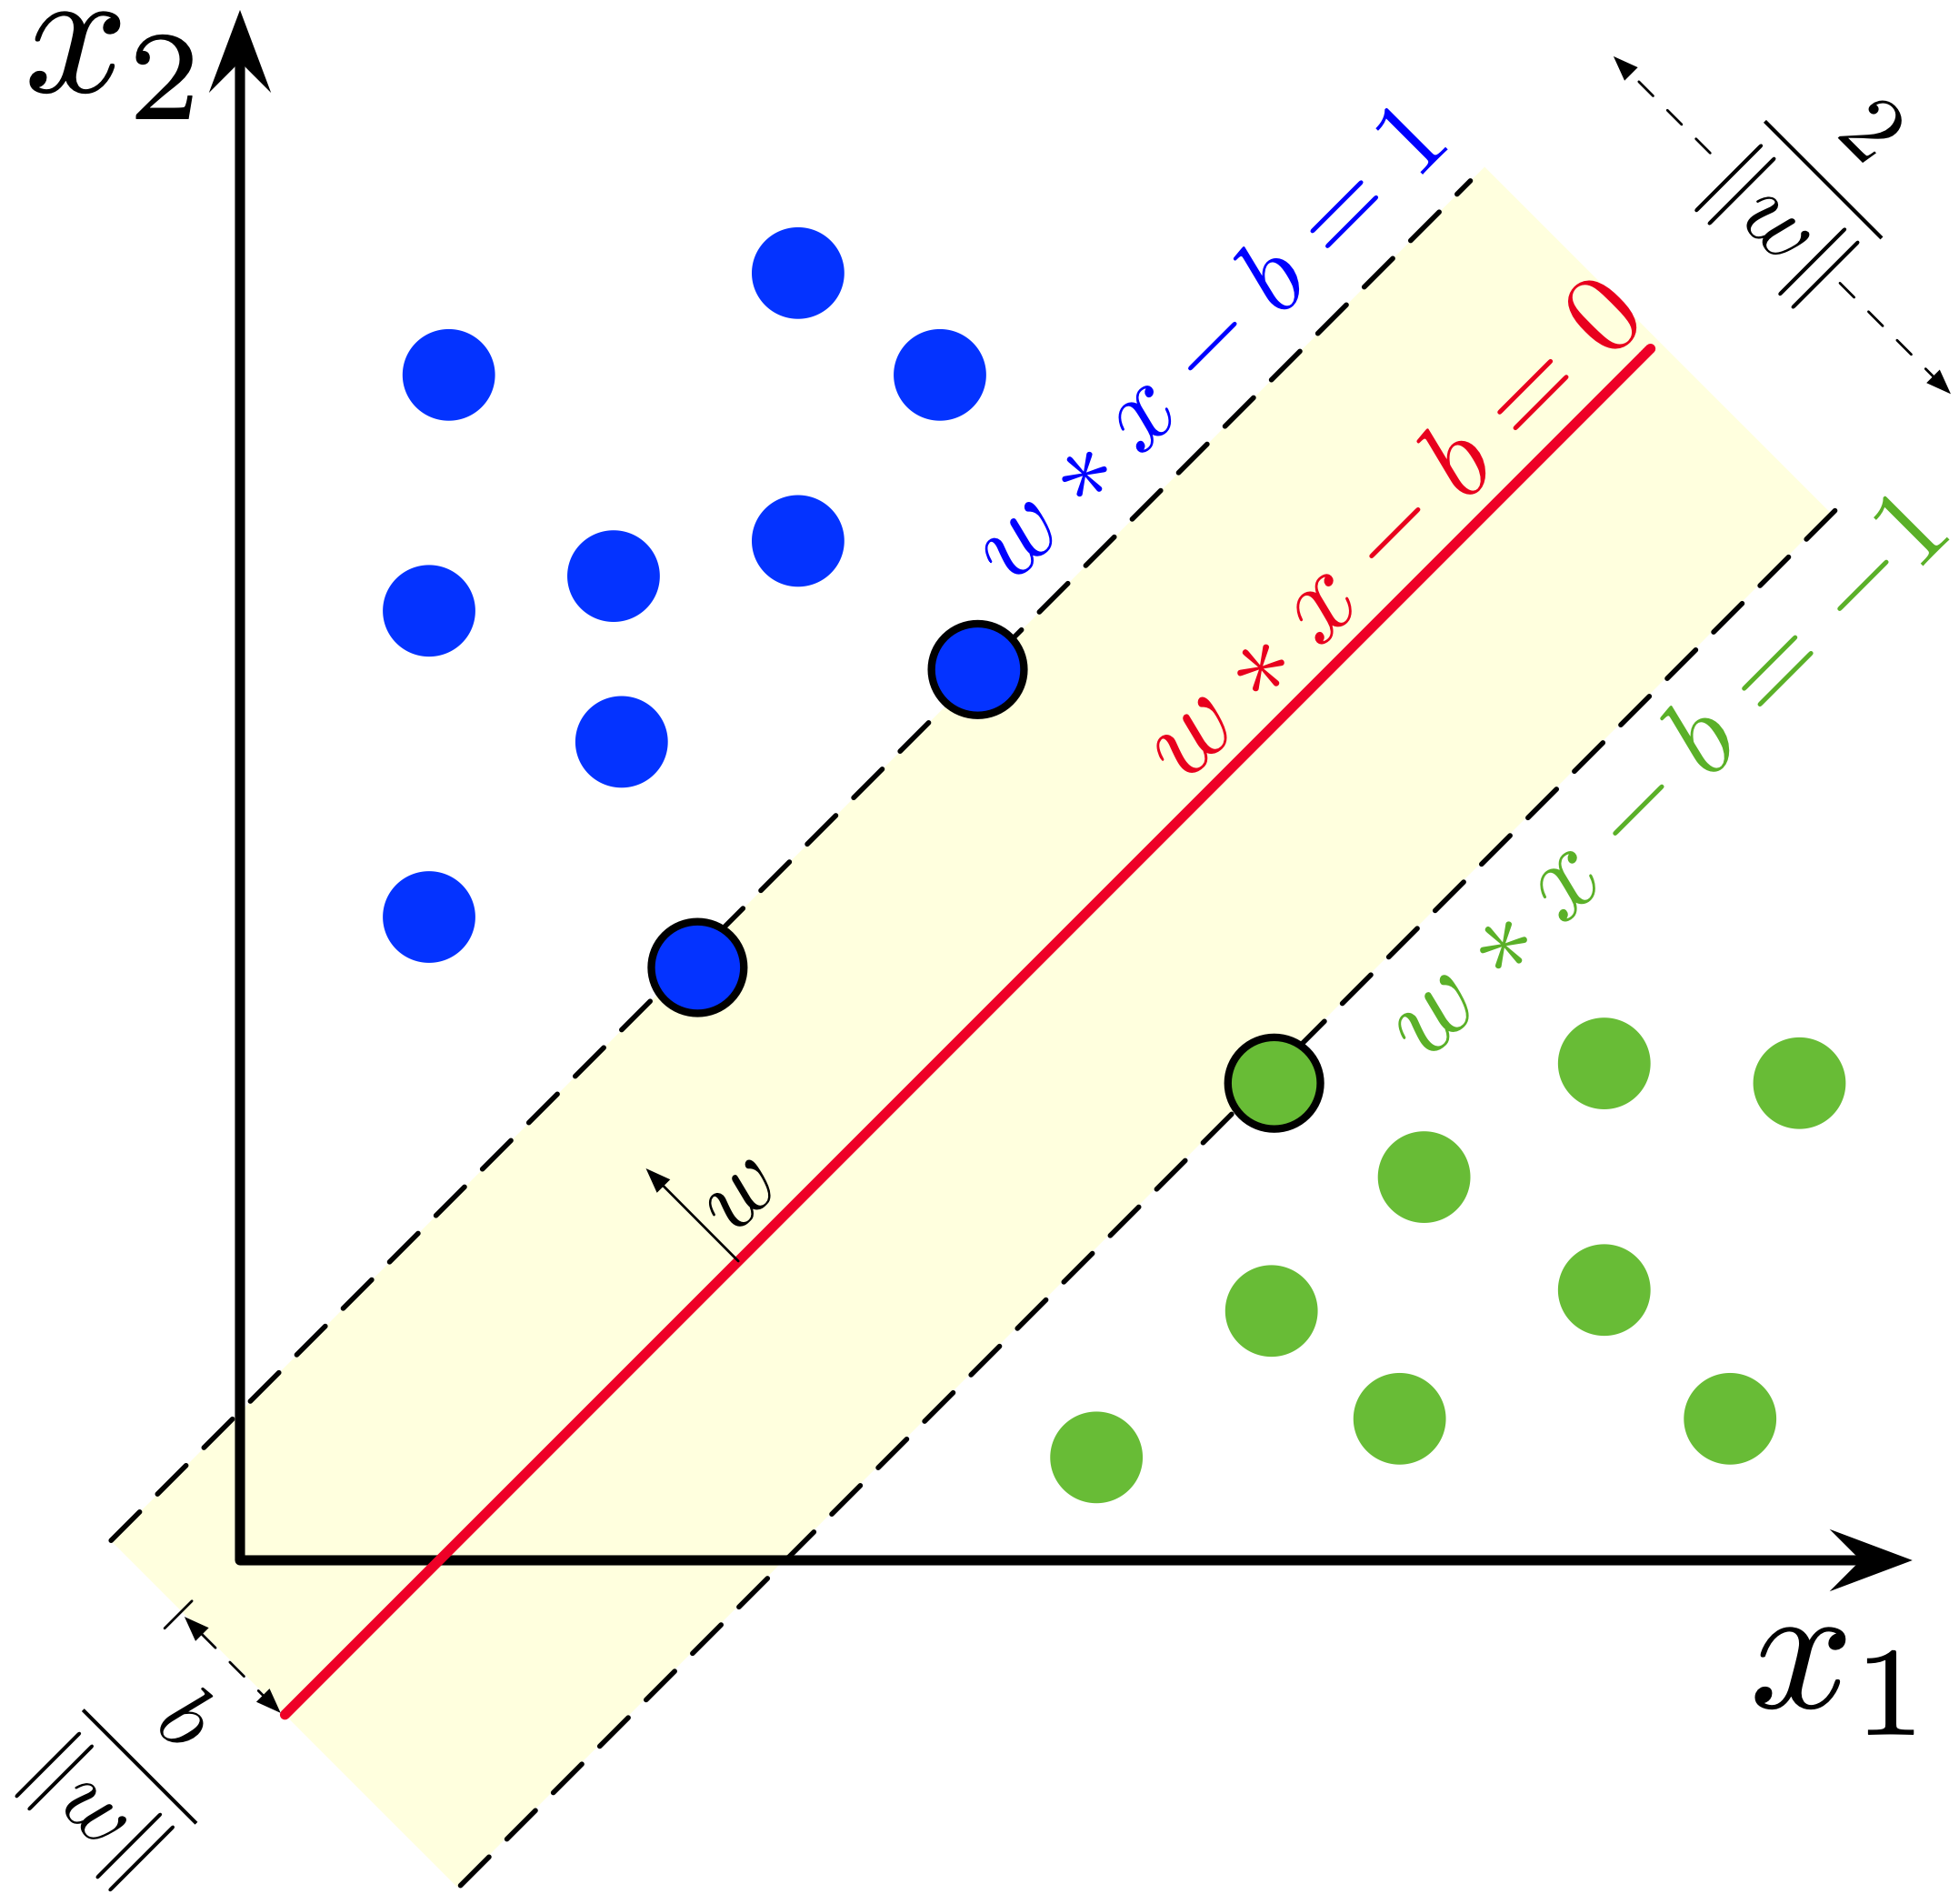
\includegraphics[height=\textheight]{FIGS/SVM_margin}
    \end{minipage}
    \begin{minipage}{0.28\textwidth}
        Maximum-margin hyperplane and margins for an SVM trained with samples from two classes. Samples on the margin are the \textbf{support vectors}
    \end{minipage}
\end{frame}

\begin{frame}
    Any \textbf{hyperplane} can be written as the set of points $\mathbf{x}$ satisfying
    \[
        \bw^\mathsf{T} \bx - b = 0
    \]
    where $\bw$ is the (not necessarily normalized) \textbf{normal vector} to the hyperplane (if the hyperplane has equation $a_1z_1+\cdots+a_pz_p=c$, then $(a_1,\ldots,a_n)$ is normal to the hyperplane)
    % \vfill
    % This is much like \textbf{Hesse normal form}, except that $\mathbf{w}$ is not necessarily a unit vector
    \vfill
    The parameter $b/\|\bw\|$ determines the offset of the hyperplane from the origin along the normal vector $\bw$
    \vfill
    Remark: a hyperplane defined thusly is not a subspace of $\IR^p$ unless $b=0$. We can of course transform the data so that it is...
\end{frame}

\begin{frame}{Linearly separable points}
    Let $X_1$ and $X_2$ be two sets of points in $\IR^p$ 
    \vfill
    Then $X_1$ and $X_2$ are \textbf{linearly separable} if there exist $w_{1}, w_{2},..,w_{p}, k\in\IR$ such that 
    \begin{itemize}
        \item every point $x \in X_1$ satisfies $\sum^{p}_{i=1} w_{i}x_{i} > k$ 
        \item every point $x \in X_2$ satisfies $\sum^{p}_{i=1} w_{i}x_{i} < k$
    \end{itemize}
    where $x_{i}$ is the $i$th component of $x$
\end{frame}

\begin{frame}{Hard-margin SVM}
    If the training data is \textbf{linearly separable}, we can select two parallel hyperplanes that separate the two classes of data, so that the distance between them is as large as possible 
    \vfill
    The region bounded by these two hyperplanes is called the ``margin'', and the maximum-margin hyperplane is the hyperplane that lies halfway between them
    \vfill
    With a normalized or standardized dataset, these hyperplanes can be described by the equations
    \begin{itemize}
        \item $\mathbf{w}^\mathsf{T} \mathbf{x} - b = 1$ (anything on or above this boundary is of one class, with label 1) 
        \item $\mathbf{w}^\mathsf{T} \mathbf{x} - b = -1$ (anything on or below this boundary is of the other class, with label -1)
    \end{itemize}
\end{frame}

\begin{frame}
    Distance between these two hyperplanes is $2/\|\bw\|$
    \vfill
    $\Rightarrow$ to maximize the distance between the planes we want to minimize $\|\bw\|$
    \vfill
    The distance is computed using the distance from a point to a plane equation
    \vfill
    We must also prevent data points from falling into the margin, so we add the following constraint: for each $i$ either
    \[
        \mathbf{w}^\mathsf{T} \mathbf{x}_i - b \ge 1 \, , \text{ if } y_i = 1
    \]
    or
    \[
        \mathbf{w}^\mathsf{T} \mathbf{x}_i - b \le -1 \, , \text{ if } y_i = -1
    \]
    \vfill
    (Each data point must lie on the correct side of the margin)
\end{frame}

\begin{frame}
    This can be rewritten as
    \[
        y_i(\mathbf{w}^\mathsf{T} \mathbf{x}_i - b) \ge 1, \quad \text{ for all } 1 \le i \le n
    \]
    or
    \[
        y_i(\mathbf{w}^\mathsf{T} \mathbf{x}_i - b)-1\geq 0, \quad \text{ for all } 1 \le i \le n
    \]
    \vfill
    We get the optimization problem:
    \begin{quote}
        Minimize $\|\mathbf{w}\|$ subject to $y_i(\mathbf{w}^\mathsf{T} \mathbf{x}_i - b)-1 \ge 0$ for $i = 1, \ldots, n$
    \end{quote}
    \vfill
    The $\mathbf{w}$ and $b$ that solve this problem determine the classifier, $\mathbf{x} \mapsto \sgn(\mathbf{w}^\mathsf{T} \mathbf{x} - b)$ where $\sgn(\cdot)$ is the \textbf{sign function}.
\end{frame}

\begin{frame}   
    The maximum-margin hyperplane is completely determined by those $\bx_i$ that lie nearest to it
    \vfill
    These $\bx_i$ are the \textbf{support vectors}
\end{frame}

\begin{frame}{Writing the goal in terms of Lagrange multipliers}
    Recall that our goal is to
    \begin{quote}
        minimize $\|\mathbf{w}\|$ subject to $y_i(\mathbf{w}^\mathsf{T} \mathbf{x}_i - b)-1 \ge 0$ for $i = 1, \ldots, n$
    \end{quote}
    \vfill
    Using Lagrange multipliers $\lambda_1,\ldots,\lambda_n$, we have the function
    \[
        L_P:=F(\bw,b\lambda_1,\ldots,\lambda_n) =
        \frac 12\|\bw\|^2 -\sum_{i=1}^n \lambda_iy_i(\bx_i\bw+b)
        +\sum_{i=1}^n\lambda_i
    \]
    \vfill
    Note that we have as many Lagrange multipliers as there are data points. Indeed, there are that many inequalities that must be satisfied
    \vfill 
    The aim is to minimise $L_p$ with respect to $\bw$ and $b$ while the derivatives of $L_p$ w.r.t. $\lambda_i$ vanish and the $\lambda_i\geq 0$, $i=1,\ldots,n$
\end{frame}

\begin{frame}{Lagrange multipliers}
    We have already seen Lagrange multipliers, when we were studying PCA
    \vfill
\end{frame}

\begin{frame}{Maximisation using Lagrange multipliers (V1.0)}
    We want the max of $f(x_1,\ldots,x_n)$ under the constraint $g(x_1,\ldots,x_n)=k$
    \begin{enumerate}
    \item Solve
    \begin{align*}
    \nabla f(x_1,\ldots,x_n) &= \lambda\nabla g(x_1,\ldots,x_n) \\
    g(x_1,\ldots,x_n) &= k
    \end{align*}
    where $\nabla=(\frac{\partial}{\partial x_1},\ldots,\frac{\partial}{\partial x_n})$ is the \textbf{gradient operator}
    \item Plug all solutions into $f(x_1,\ldots,x_n)$ and find maximum values (provided values exist and $\nabla g\neq \b0$ there)
    \end{enumerate}
    \vfill
    $\lambda$ is the \textbf{Lagrange multiplier}
\end{frame}
    
    
\begin{frame}{The gradient}
    $f:\IR^n\to\IR$ function of several variables, $\nabla=\left(\frac{\partial}{\partial x_1},\ldots,\frac{\partial}{\partial x_n}\right)$ the gradient operator
    \vfill
    Then
    \[
    \nabla f = \left(
    \frac{\partial}{\partial x_1}f,\ldots,
    \frac{\partial}{\partial x_n}f
    \right)
    \]
    \vfill
    So $\nabla f$ is a \emph{vector-valued} function, $\nabla f:\IR^n\to\IR^n$; also written as
    \[
    \nabla f = f_{x_1}(x_1,\ldots,x_n)\be_1+\cdots f_{x_n}(x_1,\ldots,x_n)\be_n
    \]
    where $f_{x_i}$ is the partial derivative of $f$ with respect to $x_i$ and $\{\be_1,\ldots,\be_n\}$ is the standard basis of $\IR^n$
\end{frame}

\begin{frame}{Lagrange multipliers (V2.0)}
        However, the problem we were considering then involved a single multiplier $\lambda$
        \vfill
        Here we want $\lambda_1,\ldots,\lambda_n$
\end{frame}

\begin{frame}{Lagrange multiplier theorem}
    \begin{theorem}
        Let $f\colon\mathbb{R}^n \rightarrow \mathbb{R}$ be the objective function, $g\colon\mathbb{R}^n \rightarrow \mathbb{R}^c $ be the constraints function, both being $C^1$.
        Consider the optimisation problem
        \begin{align*}
            \text{maximize}\ f(x) \\
            \text{subject to}\ g(x) = 0                 
        \end{align*}
        Let $x^*$ be an optimal solution to the optimization problem, such that $\operatorname{rank} (Dg(x^*)) = c < n$, where $Dg(x^*)$ denotes the matrix of partial derivatives
        \[
            \left[{\partial g_j}/{\partial x_k}\right]  
        \]
        Then there exists a unique Lagrange multiplier $\lambda^* \in \mathbb{R}^c$ such that
        \[
            Df(x^*) = \lambda^{*T}Dg(x^*)
        \]
    \end{theorem}
\end{frame}

\begin{frame}{Lagrange multipliers (V3.0)}
    Here we want $\lambda_1,\ldots,\lambda_n$
    \vfill
    But we also are looking for $\lambda_i\geq 0$
    \vfill 
    So we need to consider the so-called Karush-Kuhn-Tucker (KKT) conditions
\end{frame}

\begin{frame}{Karush-Kuhn-Tucker (KKT) conditions}
    Consider the optimisation problem
    \begin{align*}
        \text{maximize}\ f(x) \\
        \text{subject to}& \quad g_i(x) \leq 0  \\
        &\quad h_i(x)=0               
    \end{align*}
    Form the Lagrangian
    \[
        L(\bx,\mu,\lambda) = f(\bx)+\mu^T\bg(\bx)+\lambda^T\bh(\bx)
    \]
    \begin{theorem}
        If $(\mathbf{x}^{\ast},\mathbf{\mu}^\ast)$ is a \emph{saddle point} of $L(\mathbf{x},\mathbf{\mu})$ in $\mathbf{x} \in \mathbf{X}$, $\mathbf{\mu} \geq \mathbf{0}$, then $\mathbf{x}^{\ast}$ is an optimal vector for the above optimization problem. Suppose that $f(\mathbf{x})$ and $g_i(\mathbf{x})$, $i = 1, \ldots, m$, are \emph{convex} in $\mathbf{x}$ and that there exists $\mathbf{x}_{0} \in \mathbf{X}$ such that $\mathbf{g}(\mathbf{x}_{0}) < 0$. Then with an optimal vector $\mathbf{x}^{\ast}$ for the above optimization problem there is associated a non-negative vector $\mathbf{\mu}^\ast$ such that $L(\mathbf{x}^{\ast},\mathbf{\mu}^\ast)$ is a saddle point of $L(\mathbf{x},\mathbf{\mu})$
    \end{theorem}
\end{frame}

\begin{frame}{KKT conditions}
    \begin{align*}
        \frac{\partial}{\partial w_\nu}L_P &=
        w_\nu-\sum_{i}^n\lambda_iy_ix_{i\nu}=0
        \qquad\nu=1,\ldots,p \\
        \frac{\partial}{\partial b}L_P &=
        -\sum_{i=1}^n \lambda_iy_i = 0 \\
        y_i(\bx_i^T\bw+b)-1 &\geq 0\qquad i=1,\ldots,n \\
        \lambda_i &\geq 0\qquad i=1,\ldots,n \\
        \lambda_i(y_i(\bx_i^T\bw+b)-1) &=0\qquad i=1,\ldots,n \\
    \end{align*}
\end{frame}


\begin{frame}[fragile]\frametitle{Numerical example}
Example from \href{https://www.datacamp.com/tutorial/support-vector-machines-r}{here}
\vfill
\begin{knitrout}
\definecolor{shadecolor}{rgb}{0.969, 0.969, 0.969}\color{fgcolor}\begin{kframe}
\begin{alltt}
\hlkwd{set.seed}\hldef{(}\hlnum{10111}\hldef{)}
\hldef{x} \hlkwb{=} \hlkwd{matrix}\hldef{(}\hlkwd{rnorm}\hldef{(}\hlnum{40}\hldef{),} \hlnum{20}\hldef{,} \hlnum{2}\hldef{)}
\hldef{y} \hlkwb{=} \hlkwd{rep}\hldef{(}\hlkwd{c}\hldef{(}\hlopt{-}\hlnum{1}\hldef{,} \hlnum{1}\hldef{),} \hlkwd{c}\hldef{(}\hlnum{10}\hldef{,} \hlnum{10}\hldef{))}
\hldef{x[y} \hlopt{==} \hlnum{1}\hldef{,]} \hlkwb{=} \hldef{x[y} \hlopt{==} \hlnum{1}\hldef{,]} \hlopt{+} \hlnum{1}
\hlkwd{plot}\hldef{(x,} \hlkwc{col} \hldef{= y} \hlopt{+} \hlnum{3}\hldef{,} \hlkwc{pch} \hldef{=} \hlnum{19}\hldef{)}
\end{alltt}
\end{kframe}
\end{knitrout}
\end{frame}

\maxFrameImage{FIGS/L14-plot-svm-example-1.pdf}

\begin{frame}[fragile]
\begin{knitrout}
\definecolor{shadecolor}{rgb}{0.969, 0.969, 0.969}\color{fgcolor}\begin{kframe}
\begin{alltt}
\hldef{dat} \hlkwb{=} \hlkwd{data.frame}\hldef{(x,} \hlkwc{y} \hldef{=} \hlkwd{as.factor}\hldef{(y))}
\hldef{svmfit} \hlkwb{=} \hlkwd{svm}\hldef{(y} \hlopt{~} \hldef{.,} \hlkwc{data} \hldef{= dat,} \hlkwc{kernel} \hldef{=} \hlsng{"linear"}\hldef{,} \hlkwc{cost} \hldef{=} \hlnum{10}\hldef{,} \hlkwc{scale} \hldef{=} \hlnum{FALSE}\hldef{)}
\hlkwd{print}\hldef{(svmfit)}
\end{alltt}
\begin{verbatim}
## 
## Call:
## svm(formula = y ~ ., data = dat, kernel = "linear", cost = 10, scale = FALSE)
## 
## 
## Parameters:
##    SVM-Type:  C-classification 
##  SVM-Kernel:  linear 
##        cost:  10 
## 
## Number of Support Vectors:  6
\end{verbatim}
\begin{alltt}
\hlkwd{plot}\hldef{(svmfit, dat)}
\end{alltt}
\end{kframe}
\end{knitrout}
\end{frame}

\maxFrameImage{FIGS/L14-plot-svm-example-result-1.pdf}


\begin{frame}[fragile]
\begin{knitrout}
\definecolor{shadecolor}{rgb}{0.969, 0.969, 0.969}\color{fgcolor}\begin{kframe}
\begin{alltt}
\hldef{make.grid} \hlkwb{=} \hlkwa{function}\hldef{(}\hlkwc{x}\hldef{,} \hlkwc{n} \hldef{=} \hlnum{75}\hldef{) \{}
  \hldef{grange} \hlkwb{=} \hlkwd{apply}\hldef{(x,} \hlnum{2}\hldef{, range)}
  \hldef{x1} \hlkwb{=} \hlkwd{seq}\hldef{(}\hlkwc{from} \hldef{= grange[}\hlnum{1}\hldef{,}\hlnum{1}\hldef{],} \hlkwc{to} \hldef{= grange[}\hlnum{2}\hldef{,}\hlnum{1}\hldef{],} \hlkwc{length} \hldef{= n)}
  \hldef{x2} \hlkwb{=} \hlkwd{seq}\hldef{(}\hlkwc{from} \hldef{= grange[}\hlnum{1}\hldef{,}\hlnum{2}\hldef{],} \hlkwc{to} \hldef{= grange[}\hlnum{2}\hldef{,}\hlnum{2}\hldef{],} \hlkwc{length} \hldef{= n)}
  \hlkwd{expand.grid}\hldef{(}\hlkwc{X1} \hldef{= x1,} \hlkwc{X2} \hldef{= x2)}
\hldef{\}}
\hldef{xgrid} \hlkwb{=} \hlkwd{make.grid}\hldef{(x)}
\hldef{ygrid} \hlkwb{=} \hlkwd{predict}\hldef{(svmfit, xgrid)}
\hlkwd{plot}\hldef{(xgrid,} \hlkwc{col} \hldef{=} \hlkwd{c}\hldef{(}\hlsng{"red"}\hldef{,}\hlsng{"blue"}\hldef{)[}\hlkwd{as.numeric}\hldef{(ygrid)],} \hlkwc{pch} \hldef{=} \hlnum{20}\hldef{,} \hlkwc{cex} \hldef{=} \hlnum{.2}\hldef{)}
\hlkwd{points}\hldef{(x,} \hlkwc{col} \hldef{= y} \hlopt{+} \hlnum{3}\hldef{,} \hlkwc{pch} \hldef{=} \hlnum{19}\hldef{)}
\hlkwd{points}\hldef{(x[svmfit}\hlopt{$}\hldef{index,],} \hlkwc{pch} \hldef{=} \hlnum{5}\hldef{,} \hlkwc{cex} \hldef{=} \hlnum{2}\hldef{)}
\end{alltt}
\end{kframe}
\end{knitrout}
\end{frame}

\maxFrameImage{FIGS/L14-plot-svm-example-result-2-1.pdf}

\begin{frame}[fragile]
\begin{knitrout}
\definecolor{shadecolor}{rgb}{0.969, 0.969, 0.969}\color{fgcolor}\begin{kframe}
\begin{alltt}
\hldef{beta} \hlkwb{=} \hlkwd{drop}\hldef{(}\hlkwd{t}\hldef{(svmfit}\hlopt{$}\hldef{coefs)}\hlopt\hldef{x[svmfit}\hlopt{$}\hldef{index,])}
\hldef{beta0} \hlkwb{=} \hldef{svmfit}\hlopt{$}\hldef{rho}
\hlkwd{plot}\hldef{(xgrid,} \hlkwc{col} \hldef{=} \hlkwd{c}\hldef{(}\hlsng{"red"}\hldef{,} \hlsng{"blue"}\hldef{)[}\hlkwd{as.numeric}\hldef{(ygrid)],} \hlkwc{pch} \hldef{=} \hlnum{20}\hldef{,} \hlkwc{cex} \hldef{=} \hlnum{.2}\hldef{)}
\hlkwd{points}\hldef{(x,} \hlkwc{col} \hldef{= y} \hlopt{+} \hlnum{3}\hldef{,} \hlkwc{pch} \hldef{=} \hlnum{19}\hldef{)}
\hlkwd{points}\hldef{(x[svmfit}\hlopt{$}\hldef{index,],} \hlkwc{pch} \hldef{=} \hlnum{5}\hldef{,} \hlkwc{cex} \hldef{=} \hlnum{2}\hldef{)}
\hlkwd{abline}\hldef{(beta0} \hlopt{/} \hldef{beta[}\hlnum{2}\hldef{],} \hlopt{-}\hldef{beta[}\hlnum{1}\hldef{]} \hlopt{/} \hldef{beta[}\hlnum{2}\hldef{])}
\hlkwd{abline}\hldef{((beta0} \hlopt{-} \hlnum{1}\hldef{)} \hlopt{/} \hldef{beta[}\hlnum{2}\hldef{],} \hlopt{-}\hldef{beta[}\hlnum{1}\hldef{]} \hlopt{/} \hldef{beta[}\hlnum{2}\hldef{],} \hlkwc{lty} \hldef{=} \hlnum{2}\hldef{)}
\hlkwd{abline}\hldef{((beta0} \hlopt{+} \hlnum{1}\hldef{)} \hlopt{/} \hldef{beta[}\hlnum{2}\hldef{],} \hlopt{-}\hldef{beta[}\hlnum{1}\hldef{]} \hlopt{/} \hldef{beta[}\hlnum{2}\hldef{],} \hlkwc{lty} \hldef{=} \hlnum{2}\hldef{)}
\end{alltt}
\end{kframe}
\end{knitrout}
\end{frame}

\maxFrameImage{FIGS/L14-plot-svm-example-result-3-1.pdf}

\begin{frame}{Soft-margin SVM}
    To extend SVM to cases in which the data are not linearly separable, the \textbf{hinge loss} function is helpful
    \[
        \max\left(0, 1 - y_i(\mathbf{w}^\mathsf{T} \mathbf{x}_i - b)\right)
    \]
    \vfill
    $y_i$ is the $i$th target (i.e., in this case, 1 or -1), and $\mathbf{w}^\mathsf{T} \mathbf{x}_i - b$ is the $i$-th output
    \vfill
    This function is zero if the constraint is satisfied, in other words, if $\mathbf{x}_i$ lies on the correct side of the margin
    \vfill 
    For data on the wrong side of the margin, the function's value is proportional to the distance from the margin
\end{frame}

\begin{frame}
   
    The goal of the optimization then is to minimize
    
    \[ 
        \lambda \lVert \mathbf{w} \rVert^2 +\left[\frac 1 n \sum_{i=1}^n \max\left(0, 1 - y_i(\mathbf{w}^\mathsf{T} \mathbf{x}_i - b)\right) \right]
    \]
    
    where the parameter $\lambda > 0$ determines the trade-off between increasing the margin size and ensuring that the $\mathbf{x}_i$ lie on the correct side of the margin
    \vfill
    Thus, for sufficiently small values of $\lambda$, it will behave similar to the hard-margin SVM, if the input data are linearly classifiable, but will still learn if a classification rule is viable or not
\end{frame}


% Save counters for next file

% Save theorem count for next file
\end{document}
